% This is text associated with the open textbook "Open Electromagnetics"
% See immediately below for author, date
% This work is licensed under the Creative Commons Attribution-ShareAlike 4.0 International License. (CC BY SA 4.0) 
% To view a copy of the license, visit http://creativecommons.org/licenses/by-sa/4.0/

%ORB TITLE Transformers: Principle of Operation
%ORB AUTHOR 0        # S.W. Ellingson, Virginia Tech (ellingson@vt.edu)
%ORB DATE 20180807   # yyyymmdd
%ORB ABSTRACT Transformers: Principle of Operation

\label{m0031_Transformers_Principle_of_Operation} % <-- Must match name of this file and module directory name.  Don't mess with this!
\index{transformer|(}

A transformer is a device that connects two electrical circuits through a shared magnetic field.  
Transformers are used in impedance transformation, voltage level conversion, circuit isolation, conversion between single-ended and differential signal modes, and other applications.\footnote{See ``Additional Reading'' at the end of this section for more on these applications.}
The underlying electromagnetic principle is Faraday's Law (Section~\ref{m0055_Faradays_Law}) -- in particular, transformer emf.

The essential features of a transformer can be derived from the simple experiment shown in Figures~\ref{m0031_fPoleTransformer1} and \ref{m0031_fPoleTransformer2}.  
In this experiment, two coils are arranged along a common axis.  
The winding pitch is small, so that all magnetic field lines pass through the length of the coil, and no lines pass between the windings.
To further contain the magnetic field, we assume both coils are wound on the same core, consisting of some material exhibiting high permeability. 
The upper coil has $N_1$ turns and the lower coil has $N_2$ turns. 

In Part~I of this experiment (Figure~\ref{m0031_fPoleTransformer1}), 
the upper coil is connected to a sinusoidally-varying voltage source $V_1^{(1)}$ in which the subscript refers to the coil and the superscript refers to ``Part~I'' of this experiment.
The voltage source creates a current in the coil, which in turn creates a time-varying magnetic field ${\bf B}$ in the core.  
%Applying the right-hand rule that relates current to induced magnetic field, the reference direction for ${\bf B}$ is in the downward ($-\hat{\bf z}$) direction.
%
\begin{figure}
\begin{center}
\pdftooltip{{  % note double braces
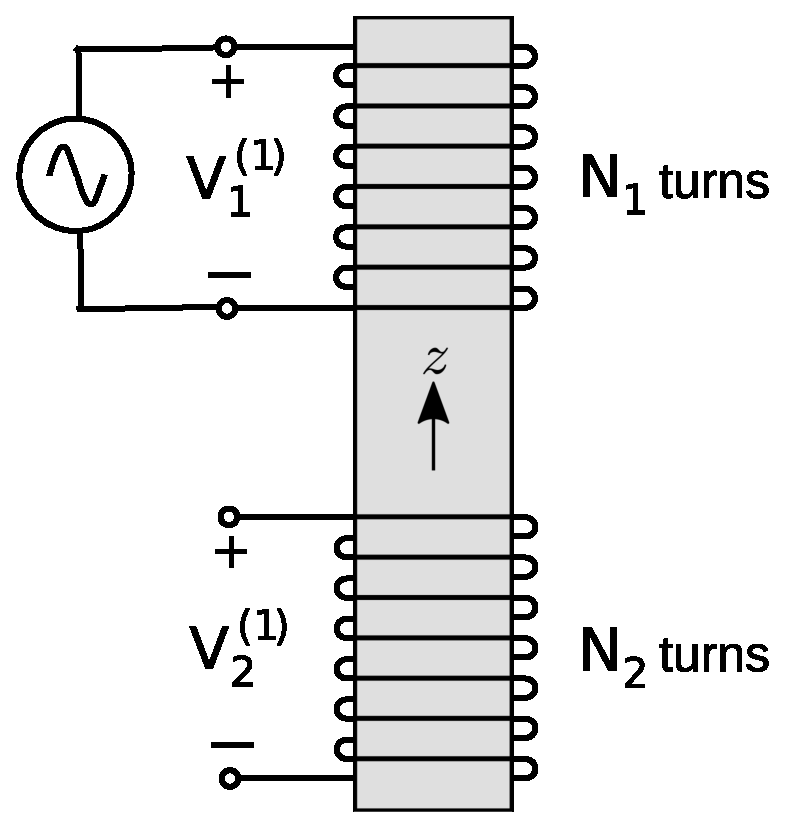
\includegraphics[width=2in]{modules/m0031_fPoleTransformer1.eps}
}}{A long rectangle with two separate groups of wire. The upper uniformly wound coil is labeled N sub 1 turns. An AC voltage source is connected to either side of the coil and labeled V sub 1 super (1). On the second coil, labeled N sub 2 turns, are 2 nodes labeled V sub 2 super (1). In both cases the positive node is above the negative node. A vector in the middle of the rectangular axis is labeled z.}
\end{center} 
\caption{\label{m0031_fPoleTransformer1} Part I of an experiment demonstrating the linking of electric circuits using a transformer.}
\end{figure}
%
\begin{figure}
\begin{center}
\pdftooltip{{  % note double braces
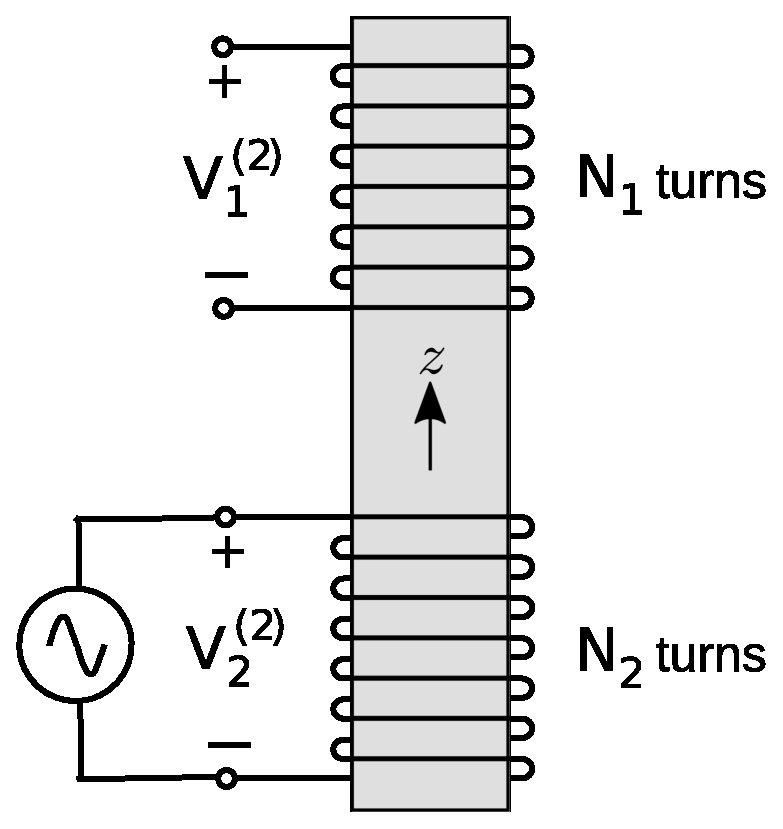
\includegraphics[width=2in]{modules/m0031_fPoleTransformer2.eps}
}}{Similar to previous figure, but flipped across the horizontal. V sub 2 is connected to an AC source and V sub 1 is an open circuit. A vector in the middle of the rectangular axis is labeled z. }
\end{center} 
\caption{\label{m0031_fPoleTransformer2} Part II of an experiment demonstrating the linking of electric circuits using a transformer.}
\end{figure} 

The lower coil has $N_2$ turns wound in the \emph{opposite direction} and is open-circuited.
Given the closely-spaced windings and use of a high-permeability core, we assume that the magnetic field within the lower coil is equal to ${\bf B}$ generated in the upper coil.  The potential induced in the lower coil is $V_2^{(1)}$ with reference polarity indicated in the figure.  
From Faraday's Law we have
%
\begin{equation}   
V_2^{(1)} = - N_2 \frac{\partial}{\partial t} \Phi_2
\label{m0031_ePartIa}
\end{equation}
%
where $\Phi_2$ is the flux through a single turn of the lower coil.  Thus:
%
\begin{equation}   
V_2^{(1)} = -N_2 \frac{\partial}{\partial t} \int_{\mathcal{S}} { {\bf B} \cdot (-\hat{\bf z}ds) }
\label{m0031_ePartIb}
\end{equation}
%
Note that the direction of $d{\bf s}=-\hat{\bf z}ds$ is determined by the polarity we have chosen for $V_2^{(1)}$.

In Part~II of the experiment (Figure~\ref{m0031_fPoleTransformer2}), we make changes as follows. We apply a voltage $V_2^{(2)}$ to the lower coil and open-circuit the upper coil. Further, we adjust $V_2^{(2)}$ such that the induced magnetic flux density is again ${\bf B}$ -- that is, equal to the field in Part~I of the experiment.  Now we have
%
\begin{equation}   
V_1^{(2)} = - N_1 \frac{\partial}{\partial t} \Phi_1 
\end{equation}
%
which is
%
\begin{equation}   
V_1^{(2)} = -N_1 \frac{\partial}{\partial t} \int_{\mathcal{S}} { {\bf B} \cdot (+\hat{\bf z}ds) }
\end{equation}
%
For reasons that will become apparent in a moment, let's shift the leading minus sign into the integral.  We then have
%
\begin{equation}   
V_1^{(2)} = +N_1 \frac{\partial}{\partial t} \int_{\mathcal{S}} { {\bf B} \cdot (-\hat{\bf z}ds) }
\end{equation}
%
Comparing this to Equations~\ref{m0031_ePartIa} and \ref{m0031_ePartIb}, we see that we may rewrite this in terms of the flux in the lower coil in Part~I of the experiment:
%
\begin{equation}   
V_1^{(2)} = +N_1 \frac{\partial}{\partial t} \Phi_2
\end{equation}
%
In fact, we can express this in terms of the \emph{potential} in Part~I of the experiment:
%
\begin{flalign}   
V_1^{(2)} &= \left(-\frac{N_1}{N_2}\right) \left(-N_2 \frac{\partial}{\partial t} \Phi_2 \right) \nonumber \\
          &= \left(-\frac{N_1}{N_2}\right) V_2^{(1)} 
\end{flalign}
%
We have found that the potential in the upper coil in Part~II is related in a simple way to the potential in the lower coil in Part~I of the experiment.
If we had done Part~II first, we would have obtained the same result but with the superscripts swapped.  
Therefore, it must be generally true -- regardless of the arrangement of terminations -- that 
%
\begin{equation}   
V_1 = -\frac{N_1}{N_2}V_2
\end{equation}
%
This expression should be familiar from elementary circuit theory -- except possibly for the minus sign.
The minus sign is a consequence of the fact that the coils are wound in opposite directions.  
We can make the above expression a little more general as follows:  
%
\begin{equation}   
\boxed{
\frac{V_1}{V_2} = p\frac{N_1}{N_2}
}
\label{m0031_eTL}
\end{equation}
%
where $p$ is defined to $+1$ when the coils are wound in the same direction and $-1$ when coils are wound in opposite directions. 
(It is an excellent exercise to confirm that this is true by repeating the above analysis with winding direction changed for either the upper or lower coil, for which $p$ will then turn out to be $+1$.)  
This is the ``transformer law'' of basic electric circuit theory, from which all other characteristics of transformers as two-port circuit devices can be obtained (See Section~\ref{m0032_Transformers_as_Two-Port_Devices} for follow-up on that).  
Summarizing:
%
%ORB HIGHLIGHT
\begin{mdframed}[backgroundcolor=yellow!20,nobreak=true] 
The ratio of coil voltages in an ideal transformer is equal to the ratio of turns with sign determined by the relative directions of the windings, per Equation~\ref{m0031_eTL}.
\end{mdframed}

A more familiar transformer design is shown in Figure~\ref{m0031_fTransformer3d_col3} -- coils wound on a toroidal core as opposed to a cylindrical core.
Why do this?
This arrangement confines the magnetic field linking the two coils to the core, as opposed to allowing field lines to extend beyond the device.
This confinement is important in order to prevent fields originating outside the transformer from interfering with the magnetic field linking the coils, which would lead to electromagnetic interference (EMI)
\index{electromagnetic interference (EMI)}
and electromagnetic compatibility (EMC) 
\index{electromagnetic compatibility (EMC)}
problems.
The principle of operation is in all other respects the same.
%
\begin{figure}
\begin{center}
\pdftooltip{{  % note double braces
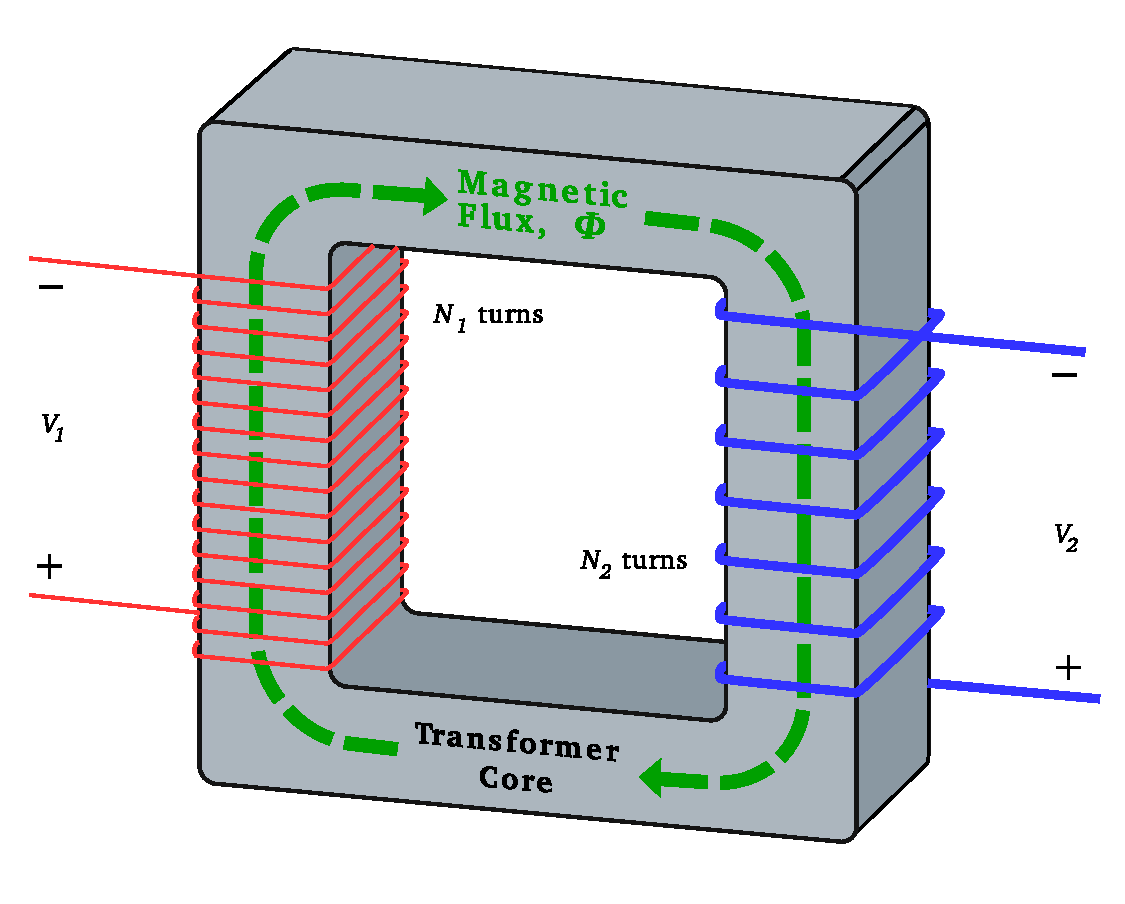
\includegraphics[width=\columnwidth]{modules/m0031_fTransformer3d_col3.eps}
% https://commons.wikimedia.org/wiki/File:Transformer3d_col3.svg
}}{A three dimensional cube with the middle cut out, representing a toroidal core and at the bottom labeled "Transformer Core". Within the core is a green dashed arrow going all the way around, pointed in a clockwise direction and labeled magnetic flux, Phi. On the left side of the core is a red coil with thin, uniform, N sub 1 turns. The top end is negative, and the bottom is positive. Between the ends is labeled V sub 1. On the right side of the core is a blue coil with more widely spaced, uniform N sub 2 turns. The top end is negative, and the bottom is positive. Between the ends is labeled V sub 2. }
\end{center} 
\centerline{\scriptsize 
\copyright~\hyperref[m0031_fTransformer3d_col3_Credit]{BillC} (modified) 
\href{https://creativecommons.org/licenses/by-sa/3.0/}{CC BY~SA 3.0} 
} 
\caption{
\label{m0031_fTransformer3d_col3}
Transformer implemented as coils sharing a toroidal core.  Here $p=+1$.
}
\end{figure}

%%%%%%%%%%%%%%%%%%%%%%%%%%%%%%%%%%%%%%%%%%%%%%%%%%%%%%%%%%%%%%%%%%%%%%

{\bf Additional Reading:}
\begin{itemize}
\item ``\href{https://en.wikipedia.org/wiki/Transformer}{Transformer}'' on Wikipedia.
\item ``\href{https://en.wikipedia.org/wiki/Balun}{Balun}'' on Wikipedia.
\end{itemize}

\index{transformer|)}
